\renewcommand*\chapterpagestyle{scrheadings}
\chapter{Results} \setAuthor{Fabian Schätzschock}

\section{Future Plans}
This section discusses future plans outside the scope of this diploma thesis,
meaning possible improvements or extensions to the system.

    \subsection{Circumventing the ESP-NOW Peer Limit}
    To circumvent the 20 peer limit per ESP, the bridge can dynamically
    dedicate another peer to act as a second bridge should the
    need arise. This would theoretically allow for infinite scalability in terms
    of Nodes. Implementing this feature would require major refactoring to the
    bridge's codebase.

    \subsection{Hot-swapping Modules}
    Currently, the modules are determined at boot time. It is possible to run
    a thread that periodically checks the connected module and activates/deactivates 
    the corresponding thread. This would allow for true hot-swapping of modules.

    \subsection{Database}
    Currently, data can only be fetched from the bridge node.
    A future improvement would be to implement a database on the
    server that stores all data. This would allow for more 
    complex queries and data analysis.

\section{Node Range Tests}
The range of the nodes was tested in a real-world scenario.
To quantify the results, the RSSI value was used. The RSSI value
is a measure of the received signal strength. The closer the value is to 0,
the stronger the signal. The RSSI value is measured in dBm.

    \subsection{Measuring Procedure}
    The range of the nodes was tested by placing a Node at a fixed location
    and walking away from it. 
    The test was conducted in two different environments:
    \begin{enumerate}
        \item An open field
        \item A 3-story apartment building
    \end{enumerate}

    The stationary Node was programmed to periodically send a
    message to the other one. The other Node was programmed to
    respond to the message. After the message was received,
    the time it took to receive the message and the 
    signal strength was recorded. 
    This process was repeated for averaging ten times.

    \subsection{Open Field}
    The open field test was conducted in a field with no obstacles
    and up to a distance of 160m.
    \vspace{1cm}

    \begin{table}[h!]
        \centering
        \begin{minipage}{0.40\textwidth} % Adjust width as needed
            \centering
            \begin{tabular}{|p{2cm}|p{1.6cm}|p{1.6cm}|}
                \hline
                \textbf{Distance (m)} & \textbf{RSSI (dBm)} & \textbf{Latency (ms)} \\ \hline
                10  & -65 & 4 \\ \hline
                20  & -80 & 5 \\ \hline
                30  & -77 & 4 \\ \hline
                40  & -88 & 5 \\ \hline
                60  & -90 & 6 \\ \hline
                80  & -83 & 6 \\ \hline
                100 & -89 & 4 \\ \hline
                160 & -89 & 4 \\ \hline
            \end{tabular}
            \label{tab:node_range_test}
        \end{minipage}%
        \hfill % Adds horizontal space between the table and figure
        \begin{minipage}{0.55\textwidth} % Adjust width as needed
            \centering
            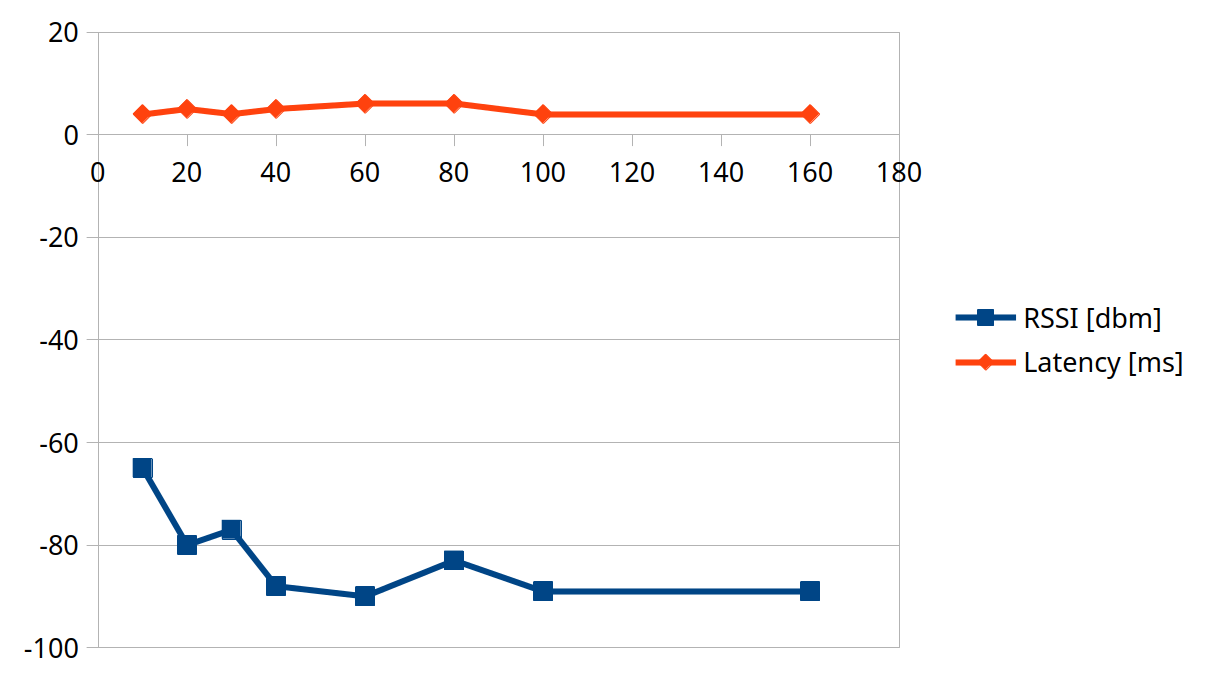
\includegraphics[width=\textwidth]{openFieldTest.png}
            \label{fig:node_range_test}
        \end{minipage}
        \caption{Node Range Test Results in an Open Field}
    \end{table}

    \subsection{Indoor Test}
    The indoor test was conducted in a 3-story apartment building.
    The Node was placed on the top floor and the second Node was
    moved further down the building. Every floor is approximately
    4m high. The test was conducted up to a distance of 12m, meaning 
    3 stories down and three ceilings in between Nodes.
    \vspace{1cm}

    \begin{table}[H]
        \centering
        \begin{minipage}{0.40\textwidth} % Adjust width as needed
            \centering
            \begin{tabular}{|p{2cm}|p{1.6cm}|p{1.6cm}|}
                \hline
                \textbf{Distance (m)} & \textbf{RSSI (dBm)} & \textbf{Latency (ms)} \\ \hline
                4   & -74 & 11 \\ \hline
                8   & -84 & 22 \\ \hline
                12  & -89 & 21 \\ \hline
            \end{tabular}
            \label{tab:node_range_test}
        \end{minipage}%
        \hfill % Adds horizontal space between the table and figure
        \begin{minipage}{0.55\textwidth} % Adjust width as needed
            \centering
            \includegraphics[width=\textwidth]{ClosedDoorTest.png}
            \label{fig:node_range_test}
        \end{minipage}
        \caption{Node Range Test Results indoors}
    \end{table}

